\chapter{The Downside Floor}

This chapter works from a short School of Hard Knocks interview segment curated by LazyingArt LLC through Video2Book. The speaker is asked about risk across his career, not about one isolated gamble. His answer gives us a compact piece of entrepreneurial reasoning: before deciding whether a risk is worth taking, we first ask what failure really leads to. In this case, the speaker's answer is stark and practical. If the venture failed, he could get a job. The comparison then shifts from fear of failure to the cost of never trying.

\section{Risk As A Career Pattern}

The interviewer begins broadly: how important was risk throughout the speaker's career? He then sharpens the question by saying that he does not mean just one instance, but the general pattern of taking risks.

That matters for the notes. We are not looking at a single heroic anecdote. We are looking at a rule of judgment. Let us name the two paths:
\begin{equation}
T = \text{try the venture},
\qquad
N = \text{do not try}.
\end{equation}
This notation is not in the interview. It is a compact way to keep the speaker's comparison visible. The spoken material is plain: he is deciding whether to act under uncertainty.

\section{The Downside Floor}

The speaker's first move is not to calculate the upside. It is to define the worst credible downside. His risk mentality at the time was that the worst thing that could happen was that he would have to get a job.

Let
\[
F = \text{failure},
\qquad
J = \text{job fallback}.
\]
The central transcript-backed relation is:
\begin{equation}
F \longrightarrow J.
\end{equation}
That is the floor under the risk. Failure is not being described as painless. It is being described as recoverable.

\begin{definition}
A \emph{downside floor} is the practical lower bound a decision-maker assigns to the failure case. In this interview, the downside floor is returning to employment.
\end{definition}

The lesson is not ``ignore risk.'' It is the opposite. We take risk seriously by making the failure state explicit. Once the speaker sees the failure state as employment rather than permanent ruin, the decision becomes thinkable.

\section{Responsibility Sharpens The Claim}

The speaker then adds a detail that should not be smoothed away: he had a newborn on the way. That fact changes the emotional weight of the decision. It makes the risk less abstract and less theatrical.

\paragraph{Anecdote.}
The speaker was not describing a carefree moment with no obligations. He was taking risk while a child was coming.

\paragraph{Mechanism.}
The newborn detail does not erase the downside floor. It tests it. With responsibility present, the relevant question becomes:
\begin{equation}
\text{If this fails, is the fallback still real?}
\end{equation}
For the speaker, the answer was yes. If the venture failed, he would go get a job. Responsibility makes that fallback more important, not less.

\section{The Real Risk}

At this point the answer pivots. Because the failure path is bounded, the speaker says, in effect, that he could take the risk. The order is important: he does not begin with appetite for danger. He begins with the survivability of failure.

\subsection{Question \& Answer}

\paragraph{Question.}
Was the real risk simply that the venture might fail?

\paragraph{Answer.}
Not quite. Venture failure was a risk, but in the speaker's own framing it led back to work:
\begin{equation}
T \ \text{followed by} \ F \longrightarrow J.
\end{equation}
The more durable risk appears in the alternative path. If he did not try, he imagined himself sitting at a job later, still wondering why he never attempted it. So the no-try path also contains a job, but it contains something extra:
\begin{equation}
N \longrightarrow J + R_N,
\end{equation}
where \(R_N\) denotes the regret, counterfactual burden, or continuing question attached to not trying.

This is the hinge of the passage. The job appears on both sides of the comparison. The difference is what the job means.

\section{A Minimal Decision Calculation}

Now we can write the speaker's reasoning as a small, cautious calculation. We should not pretend that the transcript supplies probabilities, expected returns, or a full economic model. It does not. But it does give a qualitative comparison.

Let \(C_{T|F}\) be the personal cost of trying and then failing. Let \(C_N\) be the personal cost of not trying. Let \(D_J\) be the burden of ending up in a job, and let \(R_N\) be the regret attached to never making the attempt. The speaker's comparison can be reconstructed as:
\begin{align}
C_{T|F} &\approx D_J, \\
C_N &\approx D_J + R_N.
\end{align}
Subtracting the first line from the second gives:
\begin{align}
C_N - C_{T|F}
&\approx (D_J + R_N) - D_J \\
&= R_N.
\end{align}
So, within this simplified comparison,
\begin{equation}
R_N > 0
\qquad \Longrightarrow \qquad
C_N > C_{T|F}.
\end{equation}

\begin{proposition}
In the speaker's stated risk frame, if the regret of not trying is real and the failure path returns to employment, then not trying can be costlier than trying and failing.
\end{proposition}

\begin{proof}
The try-and-fail path ends at the job fallback \(J\), so its reconstructed cost is \(D_J\). The no-try path also leaves the speaker at a job, but adds the continuing burden \(R_N\). Therefore \(C_N - C_{T|F} \approx R_N\). If \(R_N>0\), the no-try path is costlier in this limited comparison.
\end{proof}

This does not prove that every venture should be attempted. It proves something narrower and more useful: once the downside is bounded, the cost of inaction must also be counted.

\begin{figure}
\centering
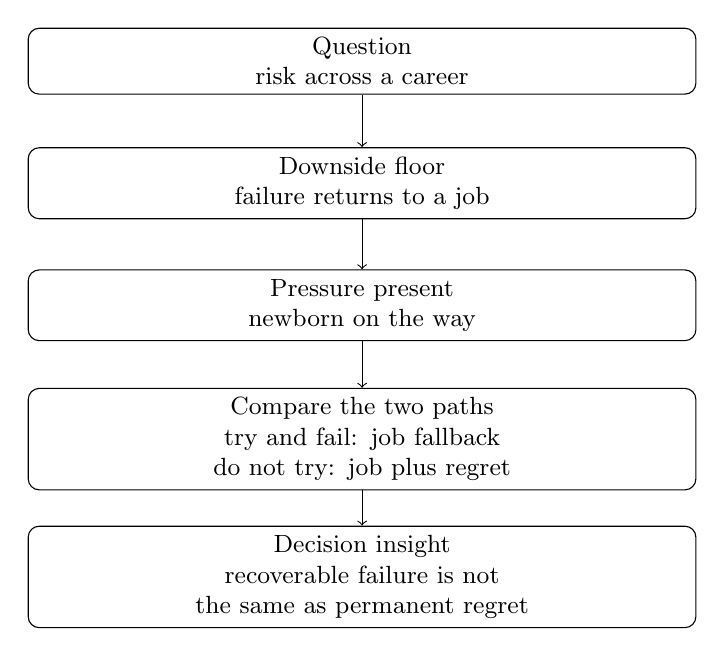
\begin{tikzpicture}[every node/.style={font=\small}]
\node[draw, rounded corners, align=center, text width=0.68\linewidth] (q) at (0,0)
{Question\\risk across a career};

\node[draw, rounded corners, align=center, text width=0.68\linewidth] (floor) at (0,-1.55)
{Downside floor\\failure returns to a job};

\node[draw, rounded corners, align=center, text width=0.68\linewidth] (pressure) at (0,-3.10)
{Pressure present\\newborn on the way};

\node[draw, rounded corners, align=center, text width=0.68\linewidth] (compare) at (0,-4.80)
{Compare the two paths\\try and fail: job fallback\\do not try: job plus regret};

\node[draw, rounded corners, align=center, text width=0.68\linewidth] (lesson) at (0,-6.55)
{Decision insight\\recoverable failure is not\\the same as permanent regret};

\draw[->] (q) -- (floor);
\draw[->] (floor) -- (pressure);
\draw[->] (pressure) -- (compare);
\draw[->] (compare) -- (lesson);
\end{tikzpicture}
\caption{A compact reconstruction of the speaker's sequence: career-wide risk, bounded downside, responsibility, and the comparison between failure and inaction.}
\end{figure}

\section{The Cost Of Not Trying}

The final sentence of the excerpt completes the argument. The speaker says that if he did not try, he would be sitting at a job somewhere, always wondering why he had not attempted it.

That is the point at which risk becomes opportunity cost. The same destination, employment, appears in both cases, but with different meanings:
\begin{align}
\text{try, fail} &\longrightarrow \text{job as fallback}, \\
\text{do not try} &\longrightarrow \text{job as regret site}.
\end{align}
This is why the speaker's answer belongs in a chapter on entrepreneurial judgment rather than a chapter on boldness. The claim is not that risk is automatically good. The claim is that a founder must compare the true failure path with the true inaction path.

The practical question becomes:
\begin{equation}
\text{What is the cost of failure, and what is the cost of never testing the idea?}
\end{equation}
For this speaker, the failure cost was bounded by the ability to work. The inaction cost was the possibility of carrying the unanswered question forward.

\section{Summary}

The excerpt unfolds in a tight order. First, risk is framed as a career pattern. Second, the speaker defines his downside floor: if he failed, he could get a job. Third, responsibility enters through the newborn detail, making the decision serious rather than casual. Fourth, the real comparison appears: trying and failing may return him to employment, but not trying leaves him with employment plus regret.

The durable principle is therefore careful rather than reckless:
\begin{equation}
\text{recoverable downside}
\quad \text{must be compared with} \quad
\text{durable regret of inaction}.
\end{equation}
That is the chapter's working contribution to the broader entrepreneurship book. Risk is not measured only by what can go wrong. It is also measured by what a person may have to live with if he never tries.